\documentclass[a4paper, 12pt]{article}
\usepackage{tikz, pgfplots, pgfplotstable, pgfmath-xfp}
\pgfplotsset{compat=newest}

\begin{document}
\begin{figure}[h]
    \centering
    \begin{tikzpicture}
        \pgfplotstableread[col sep=comma]{Data.csv}\tabledata
        \begin{axis}[
                xlabel = X,
                ylabel = Y,
                grid = both,
                % legend pos = north east,
            ]
            \addplot table [x=X, y=Y, col sep=comma,]{\tabledata};
        \end{axis}
    \end{tikzpicture}
\end{figure}
\pagebreak
\begin{figure}[h]
    \begin{tikzpicture}[domain=1:5]
        \draw[very thin,color=gray] (0,0) grid (10,10);
        \draw[->] (0,0) -- (11,0) node[right] {$x$};
        \draw[->] (0,0) -- (0,11) node[above] {$y$};
        \draw[color=orange] plot (\x,{exp(\x)}) node[right] {$f(x) = \frac{1}{20} \mathrm e^x$};
        \end{tikzpicture}   
\end{figure}
\end{document}